\begin{abstract}
Large language model (LLM) chat assistants are becoming an advertising
surface. The previous surface, keyword search, shipped with broken
incentives, and an industry grew to monetize the breakage; the new
surface is a chance to get the incentives provably right on day one. The
conversation embeds as a point \texttt{x} in a continuous space of
hundreds of dimensions, and each advertiser declares a center \texttt{c}
(their customer). The conceptual distance between them measures how
closely they match. A reach \(\sigma\) (how widely they serve) and a bid
\texttt{b} (what a conversion is worth) compare that distance against a
willingness to pay. The slot beside the reply goes to the advertiser
with the highest \(\log(b) - \|x-c\|^{2}/\sigma ^{2}\). The mechanism
involves no model training or response modification. We prove in Lean 4,
with zero \texttt{sorry}, that the rule's argmax allocation with Clarke
payments forms a VCG mechanism. Truthful reporting is weakly dominant,
the allocation maximizes welfare at every query point, and its
territories form a power diagram with keyword auctions as the degenerate
case. This mechanism allows an auction to sell regions of embedding
space.
\end{abstract}

\ccsdesc[500]{Theory of computation~Algorithmic game theory and mechanism design}
\ccsdesc[300]{Information systems~Computational advertising}
\ccsdesc[300]{Software and its engineering~Formal methods}

\keywords{VCG mechanism, computational advertising, power diagram, embedding space, formal verification, Lean 4}

\maketitle

\section{One-Shot Bidding}\label{one-shot-bidding}

Keyword auctions are strategically broken, and the industry monetizes
the breakage.
\href{https://www.aeaweb.org/articles?id=10.1257/aer.97.1.242}{Edelman,
Ostrovsky and Schwarz (2007)} proved that Google's Generalized
Second-Price auction has no dominant-strategy equilibrium, so your
optimal bid depends on bids you cannot see. First-price display auctions
require shading by an amount that also depends on bids you cannot see.
An autobidding industry answered, agents running machine learning
against each other to approximate what
\href{https://doi.org/10.2307/2977633}{Vickrey (1961)} made exact
sixty-five years ago in one shot: report your value, pay the
externality, done.

Ad auctions for large language models (LLMs) restart the design problem.
A user's conversation embeds to a point \texttt{x} in a real inner
product space, in practice a few hundred dimensions. Each advertiser
declares a center \texttt{c} (who their customer is), a reach \(\sigma\)
(how wide a neighborhood they serve), and a bid \texttt{b} (what a
conversion is worth). The platform scores each advertiser at \texttt{x}
and the highest score wins. The scoring rule predates this
paper.\footnote{Proposal series:
  \href{https://june.kim/power-diagrams-ad-auctions}{june.kim/power-diagrams-ad-auctions},
  \href{https://june.kim/the-price-of-relevance}{june.kim/the-price-of-relevance},
  \href{https://june.kim/keywords-are-tiny-circles}{june.kim/keywords-are-tiny-circles},
  \href{https://june.kim/marketing-speak-is-the-protocol}{june.kim/marketing-speak-is-the-protocol}.
  Implementation:
  \href{https://github.com/kimjune01/vectorspace-adserver}{github.com/kimjune01/vectorspace-adserver}.
  Simulations:
  \href{https://june.kim/relocation-fees}{june.kim/relocation-fees},
  \href{https://june.kim/relocation-fee-dividend}{june.kim/relocation-fee-dividend}.
  Demo:
  \href{https://june.kim/vectorspace-ads/}{june.kim/vectorspace-ads},
  archived as \href{https://doi.org/10.5281/zenodo.21365798}{DOI
  10.5281/zenodo.21365798}.} An \hyperref[exchange]{open-source
exchange} implements it, \hyperref[simulations]{multi-agent simulations}
probe its market dynamics, and an \hyperref[explorer]{interactive
explorer} renders the allocation live. The mechanism lacked a proof that
it deserves the trust the proposal asks for.

We supply the proof in Lean, so that trust in the mechanism reduces to
\hyperref[formalization]{running a build command}. The contribution is
one bridge lemma, \texttt{score\_eq\_log\_reportedVal}: the scoring rule
is the logarithm of the value a report implies, unconditionally.
Everything downstream is the classical VCG argument of
\href{https://doi.org/10.2307/2977633}{Vickrey (1961)},
\href{https://doi.org/10.1007/BF01726210}{Clarke (1971)}, and
\href{https://doi.org/10.2307/1914085}{Groves (1973)}, executed
formally. We also prove that the allocation is a power diagram for
arbitrary heterogeneous reaches, and that the mechanism collapses to
Vickrey's sealed-bid second-price auction at any keyword point.

\section{Model}\label{model}

An advertiser's report is a triple \((c, \sigma , b)\):

{\def\LTcaptype{none} % do not increment counter
\begin{longtable}[]{@{}
  >{\raggedright\arraybackslash}p{(\linewidth - 4\tabcolsep) * \real{0.3333}}
  >{\raggedright\arraybackslash}p{(\linewidth - 4\tabcolsep) * \real{0.3333}}
  >{\raggedright\arraybackslash}p{(\linewidth - 4\tabcolsep) * \real{0.3333}}@{}}
\toprule\noalign{}
\begin{minipage}[b]{\linewidth}\raggedright
Field
\end{minipage} & \begin{minipage}[b]{\linewidth}\raggedright
Name
\end{minipage} & \begin{minipage}[b]{\linewidth}\raggedright
The advertiser declares
\end{minipage} \\
\midrule\noalign{}
\endhead
\bottomrule\noalign{}
\endlastfoot
\(c \in  E\) & center & who their customer is, a point in embedding
space \\
\(\sigma  > 0\) & reach & how wide a neighborhood around \texttt{c} they
serve \\
\texttt{b\ \textgreater{}\ 0} & bid & what a conversion is worth to
them \\
\end{longtable}
}

Their private valuation is a triple \((c^{*}, \sigma ^{*}, v)\) of the
same shape, and each report field may differ from its starred
counterpart. The distinction is operational. Reported distance controls
which impression the advertiser wins; true distance controls whether the
person who sees the ad converts. A supplement advertiser can declare its
center on running-shoe queries, but the declaration does not turn
supplements into shoes. Its true value at query \texttt{x} remains
Gaussian around its private center:

\[\mathrm{trueVal}(x) = v \cdot  \exp(-\|x - c^{*}\|^{2} / \sigma ^{*2})\]

True value reads as margin times conversion rate: \texttt{v} is the
margin a conversion clears, and the Gaussian factor is the probability
that the lead at \texttt{x} converts. \(\sigma\) is a length scale: the
Gaussian is unnormalized, and the exponent carries no ½. The Gaussian is
strictly positive: even a badly matched impression can convert, only
with a probability that decays rapidly with semantic distance. That is
the object observed in impression advertising, not a binary relevance
label.

The Gaussian family is an approximation, and the best available one.
Embedding coordinates are not human-interpretable, so a peak and a width
are all an advertiser can meaningfully declare, and the Gaussian is the
\href{https://en.wikipedia.org/wiki/Maximum_entropy_probability_distribution}{maximum-entropy}
model of a conversion curve known only by those two. Any other decay
imports structure for which the advertiser has no evidence. The theorems
hold inside the family, and the Limits section says what stays outside
it. The platform scores reports by

\[\mathrm{score}(x) = \log(b) - \|x - c\|^{2} / \sigma ^{2}\]

and allocates each query to an argmax of score. Thus allocation uses the
reported Gaussian while utility uses the fixed true Gaussian. Changing a
report changes the impressions won, never the underlying conversion
surface. The winner pays the Clarke pivot. With a single winner per
query, the pivot has a closed form: losers pay nothing, and the winner
pays the runner-up's implied value (zero when unopposed).

\[\mathrm{payment}_w(x) = \max_{j \ne  w}  b_j \cdot  \exp(-\|x - c_j\|^{2} / \sigma _j^{2})\]

Utility is quasilinear. Impressions are opt-in opportunities. The model
does not force an advertiser into an auction it declined to enter. A
publisher may separately restrict eligibility, but that policy defines
the player set upstream and is not a second allocation mechanism in the
model. All definitions follow Nisan's mechanism-design chapter in
\href{https://doi.org/10.1017/CBO9780511800481}{Nisan, Roughgarden,
Tardos and Vazirani, eds.~(2007)}.

The scoring rule is the embedding-space member of a known family.
\href{https://doi.org/10.1145/1250910.1250918}{Lahaie and Pennock
(2007)} analyzed keyword scoring rules of the form
\(\mathrm{bid} \times  \mathrm{quality}^s\). With the score's logarithm
taken in base \(\beta\), ranking by score is ranking by
\(b \cdot  q^{\ln(\beta )}\) with quality
\(q = \exp(-\|x-c\|^{2}/\sigma ^{2})\). The log base is therefore the
squashing parameter, \(s = \ln(\beta )\), and the squashing-parameter
literature transfers intact. Sweeping the log base is the platform's
revenue-relevance dial.

\begin{figure}
\centering
\pandocbounded{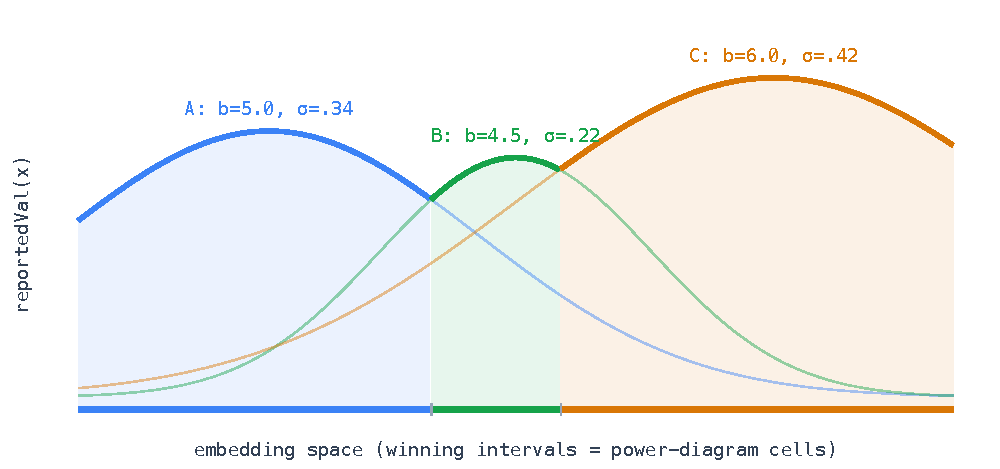
\includegraphics[keepaspectratio,alt={The allocation is the upper envelope of the reported-value curves (their logs are the score parabolas). Winning intervals along the axis are the power-diagram cells. A bid sets each curve's height, a center its position, \textbackslash sigma its width.}]{vcg-fig1.pdf}}
\caption{The allocation is the upper envelope of the reported-value
curves (their logs are the score parabolas). Winning intervals along the
axis are the power-diagram cells. A bid sets each curve's height, a
center its position, \(\sigma\) its width.}
\end{figure}

The formalization states everything over an arbitrary real inner product
space. No finite-dimension hypothesis appears anywhere in the chain. The
theorems hold for a 384-dimensional sentence embedding and for next
year's wider one alike. Drawn in one and two dimensions, the figures
show the structure that survives the trip up: cells, boundaries, argmax.
Their proportions do not survive it. In three hundred dimensions
distances concentrate and most of a cell's volume sits near its
boundary. Pictures illustrate; theorems generalize.

\section{The Bridge}\label{the-bridge}

The mechanism-design results hang on one identity. Define the value
implied by a report,
\(\mathrm{reportedVal}(x) = b \cdot  \exp(-\|x - c\|^{2}/\sigma ^{2})\).
Then

\[\mathrm{score}(x) = \log(\mathrm{reportedVal}(x))\]

with no truthfulness hypothesis (\texttt{score\_eq\_log\_reportedVal}).
The disguise is a logarithm. Log is monotone, so the argmax of score is
the argmax of reported value. The mechanism always maximizes reported
welfare, which is the allocation rule VCG requires. When a report is
truthful, reported value equals true value
(\texttt{reportedVal\_eq\_trueVal\_of\_truthful}), and the same identity
becomes \texttt{score\ =\ log(trueVal)}
(\texttt{score\_eq\_log\_trueVal}). The winner is the advertiser who
values the impression most (\texttt{winner\_maximizes\_welfare}).

\section{Weakly Dominant Strategy}\label{weakly-dominant-strategy}

\subsection{The Incentive Theorem}\label{the-incentive-theorem}

\texttt{vcg\_dsic} is the main incentive theorem: for any deviation
report \texttt{r\textquotesingle{}}, truthful reporting yields at least
the utility of reporting \texttt{r\textquotesingle{}}, regardless of
what every other player reports. The Clarke payment depends only on
others' reported values, so a player's report moves their allocation and
never their price schedule (\texttt{welfareOthersWithout\_invariant});
the four-case comparison then closes the argument. A false center can
make the supplement advertiser win the running-shoe impression, but its
utility still contains the small true supplement-conversion value, while
its payment equals the value of the shoe advertiser it displaced. In the
figure's instance, the supplement advertiser S's books at the shoe query
\texttt{x}:

{\def\LTcaptype{none} % do not increment counter
\begin{longtable}[]{@{}lll@{}}
\toprule\noalign{}
S's ledger at \texttt{x} & truthful & false center \\
\midrule\noalign{}
\endhead
\bottomrule\noalign{}
\endlastfoot
allocation & loses \texttt{x} & wins \texttt{x} \\
earns (true value at \texttt{x}) & 0 & 0.08 \\
pays (Clarke pivot) & 0 & 1.25 \\
utility & 0 & −1.17 \\
\end{longtable}
}

With one rival the pivot is the rival's reported value, so a winner's
utility is its maximum willingness to pay at \texttt{x} less what the
competitor's report says the impression is worth. The accounting
generalizes: the same four rows settle any deviation, in any dimension,
against any number of rivals, in one shot. \texttt{vcg\_dsic} is this
table quantified over all of them.

\begin{figure}
\centering
\pandocbounded{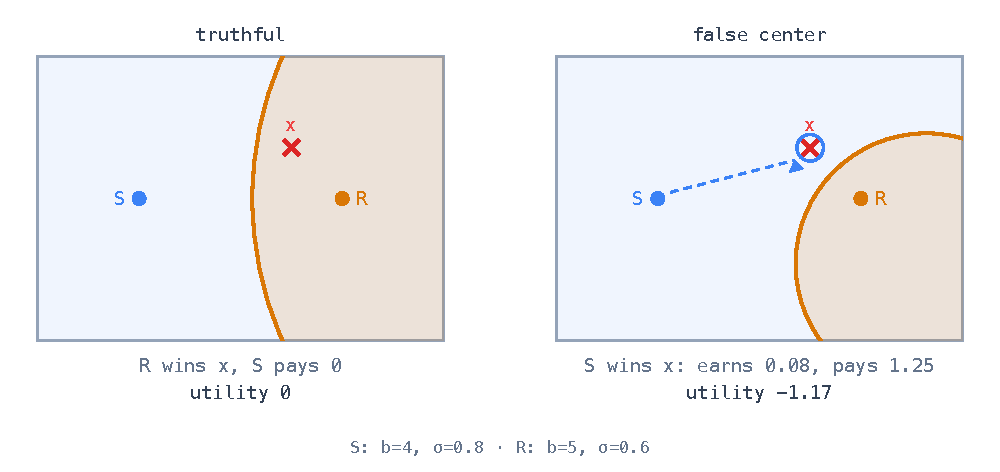
\includegraphics[keepaspectratio,alt={A false-center deviation, supplement advertiser S against running-shoe advertiser R. Left: truthful reports; the query x sits in R's cell, S pays nothing there. Right: S declares x as its center and wins it, earning its true value there (0.08) while paying R's displaced value (1.25). The deviation nets a strict loss; the ledger is vcg\_strict\_at\_contested\_point in miniature.}]{vcg-fig4.pdf}}
\caption{A false-center deviation, supplement advertiser S against
running-shoe advertiser R. Left: truthful reports; the query x sits in
R's cell, S pays nothing there. Right: S declares x as its center and
wins it, earning its true value there (0.08) while paying R's displaced
value (1.25). The deviation nets a strict loss; the ledger is
\protect\texttt{vcg\_strict\_at\_contested\_point} in miniature.}
\end{figure}

\texttt{vcg\_dsic} proves more than the informal claim usually attached
to VCG. The truthfulness it certifies constrains all three report
fields: center, reach, and bid. Misreporting your center toward a
traffic hotspot is a deviation \texttt{r\textquotesingle{}} like any
other, and the theorem says it cannot profit you.

\subsection{Observational Equivalence}\label{observational-equivalence}

Weak dominance does not by itself identify the literal report. In a thin
market, an unopposed winner pays zero, and every center report that
preserves its allocation gives the same utility.
\hyperref[formalization]{The artifact} proves the limiting case
explicitly, with pointwise and expected utility invariant under every
report when only one player competes
(\texttt{playerUtility\_invariant\_of\_subsingleton},
\texttt{expectedPlayerUtility\_invariant\_of\_subsingleton}).

Competition closes that gap. A center deviation that crosses a contested
allocation boundary sacrifices true surplus and is strictly worse
(\texttt{vcg\_strict\_at\_contested\_point}), and when the disagreement
covers a positive-weight region the loss survives aggregation
(\texttt{vcg\_strict\_expected\_on\_allocation\_change\_set}).
Observational equivalence remains: reports that preserve allocation
where competition matters. An expected-utility tie cannot place positive
query weight on queries where the allocations disagree and the deviation
is strictly worse
(\texttt{expected\_utility\_tie\_disagreement\_not\_positive}). Finite
weighted query logs construct the required strictness witness whenever
that set contains a logged query of positive weight.

\subsection{Spatial Competition}\label{spatial-competition}

The strictness theorems answer the most immediate Hotelling objection.
In spatial competition from
\href{https://doi.org/10.2307/2224214}{Hotelling (1929)} onward, sellers
drift toward the center of the market, and the analogue in embedding
space is advertisers declaring centers near high-traffic regions. VCG
makes truthful center reporting weakly dominant, so Hotelling drift
cannot increase advertiser utility. Competition converts false spatial
proximity from a costless declaration into a strictly costly allocation
error. A reported center changes placement but not customer fit: the
supplement advertiser from that ledger still earns its small true value
while paying for the shoe advertiser it displaces. As rival coverage
thickens, the allocation-equivalent class can contract toward the
advertiser's true center. Under the artifact's explicit spatial-coverage
condition, every selection from that surviving class converges to
\texttt{c*} (\texttt{centers\_converge\_of\_competitive\_coverage}). The
convergence result is conditional rather than a claim about adjustment
dynamics, and profitable drift can return through what the model
excludes: budgets, volume-dependent objectives, endogenous products or
creatives, and non-Gaussian true values.

\subsection{Comparison with Alternative
Mechanisms}\label{comparison-with-alternative-mechanisms}

The qualifier earns its value in comparison. GSP gives keyword bidders
no dominant strategy
(\href{https://www.aeaweb.org/articles?id=10.1257/aer.97.1.242}{Edelman,
Ostrovsky and Schwarz, 2007}), and even an exact second-price keyword
auction makes only the bid truthful: keyword selection and match types
remain strategic choices made against unobserved rivals, so targeting
sits outside the incentive guarantee. In the present mechanism targeting
is part of the report, and the guarantee covers it. The same comparison
orders the LLM mechanisms:

{\def\LTcaptype{none} % do not increment counter
\begin{longtable}[]{@{}
  >{\raggedright\arraybackslash}p{(\linewidth - 8\tabcolsep) * \real{0.2000}}
  >{\raggedright\arraybackslash}p{(\linewidth - 8\tabcolsep) * \real{0.2000}}
  >{\raggedright\arraybackslash}p{(\linewidth - 8\tabcolsep) * \real{0.2000}}
  >{\raggedright\arraybackslash}p{(\linewidth - 8\tabcolsep) * \real{0.2000}}
  >{\raggedright\arraybackslash}p{(\linewidth - 8\tabcolsep) * \real{0.2000}}@{}}
\toprule\noalign{}
\begin{minipage}[b]{\linewidth}\raggedright
Mechanism
\end{minipage} & \begin{minipage}[b]{\linewidth}\raggedright
Truthful report
\end{minipage} & \begin{minipage}[b]{\linewidth}\raggedright
Allocation
\end{minipage} & \begin{minipage}[b]{\linewidth}\raggedright
Welfare
\end{minipage} & \begin{minipage}[b]{\linewidth}\raggedright
Proof
\end{minipage} \\
\midrule\noalign{}
\endhead
\bottomrule\noalign{}
\endlastfoot
GSP (keywords) & \emph{none exists} & deterministic &
\emph{unguaranteed} & --- \\
Vickrey (keywords) & bid only; \emph{targeting strategic} &
deterministic & \emph{per conflated bin} & classical \\
MOSAIC & reward function & \emph{randomized softmax} &
\emph{approximate} & paper \\
Retrieval-time & \emph{bid only} & \emph{probabilistic draw} &
\emph{unguaranteed} & paper \\
LLM-Auction (training) & \emph{no report to state} & \emph{weights,
opaque} & \emph{unstated} & \emph{none} \\
\textbf{Power diagram} & bid, center, reach & deterministic argmax &
exact, pointwise & Lean, zero \texttt{sorry} \\
\end{longtable}
}

Italics mark the concessions.

\section{Geometry}\label{geometry}

The name ``power diagram auction'' is now a theorem: in \texttt{E} when
advertisers share a reach, and in \(E \times  \mathbb{R}\) when they do
not.

\subsection{Equal Reach}\label{equal-reach}

When two advertisers share \(\sigma\), comparing scores at \texttt{x} is
comparing power distances \(\|x - c\|^{2} - w\) with sites at the
centers and weights \(w = \sigma ^{2} \log(b)\)
(\texttt{score\_le\_iff\_powerDist\_le}). The score difference is an
affine function of \texttt{x} (\texttt{score\_sub\_affine}), so cell
boundaries are hyperplanes. That is the classical power diagram of
\href{https://doi.org/10.1137/0216006}{Aurenhammer (1987)}, with bids
setting the weights. When every advertiser shares \(\sigma\), the winner
rule is that cell assignment in \texttt{E} directly: the argmax of score
minimizes power distance (\texttt{winner\_minimizes\_powerDist}). No
lift required.

\subsection{Heterogeneous Reach}\label{heterogeneous-reach}

With distinct \(\sigma\)s the in-space boundaries curve, and the folk
description of the allocation as a power diagram fails in \texttt{E}. It
succeeds in \(E \times  \mathbb{R}\). Lift each query to the paraboloid
\((x, \|x\|^{2})\). Each report \((c, \sigma , b)\) determines a lifted
site and weight under which maximizing score is minimizing lifted power
distance. The auction's winner rule is then the lifted diagram's cell
assignment (\texttt{liftedPowerDist\_paraboloid},
\texttt{score\_le\_iff\_liftedPowerDist\_ge},
\texttt{winner\_minimizes\_liftedPowerDist}; the site and weight
formulas are in PowerDiagram.lean). Aurenhammer proved diagrams of
quadratic distance functions lift this way; the formalization
instantiates his lift for this scoring rule and checks the algebra once.
\hyperref[explorer]{The explorer} renders the cells live. Exact O(log N)
point location is a fixed-low-dimension result and does not survive
embedding dimension, but the lift still pays at serving time. Score
comparisons are affine in the lifted query \((x, \|x\|^{2})\). So
finding the winner is a maximum-inner-product search against static
lifted sites, which approximate-nearest-neighbor indexes and cache
layers serve sublinearly in practice, with the O(N) scan as the exact
fallback.

\begin{figure}
\centering
\pandocbounded{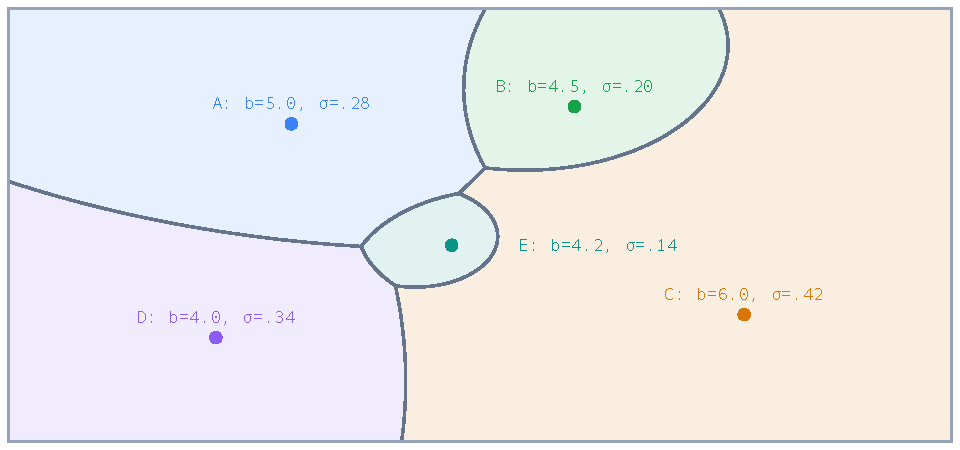
\includegraphics[keepaspectratio,alt={Five advertisers with unequal reach. Tight specialists carve bubbles out of wider generalists, and adjacent cells meet in circular arcs. The boundaries are flat only upstairs: quadric bisectors in E are hyperplanes in E \textbackslash times \textbackslash mathbb\{R\}.}]{vcg-fig2.pdf}}
\caption{Five advertisers with unequal reach. Tight specialists carve
bubbles out of wider generalists, and adjacent cells meet in circular
arcs. The boundaries are flat only upstairs: quadric bisectors in E are
hyperplanes in E \(\times\) \(\mathbb{R}\).}
\end{figure}

\section{Keywords Recovered}\label{keywords-recovered}

The migration path follows from the geometry: a keyword is a tiny
circle, a report whose reach has shrunk to a point. Keyword auctions are
the degenerate case of the embedding auction, so the general mechanism
is backward compatible: adopting it strands no existing buyer. The claim
is now a theorem pair.

\subsection{\texorpdfstring{The \(\sigma\) \(\rightarrow\) 0
Limit}{The \textbackslash sigma \textbackslash rightarrow 0 Limit}}\label{the-sigma-rightarrow-0-limit}

At any point other than its center, a report's score diverges to
\(-\infty\) as \(\sigma  \to  0\), while its score at the center is
\texttt{log(b)} independent of \(\sigma\)
(\texttt{keyword\_is\_degenerate\_limit}, \texttt{score\_at\_center}).
The tiny circle collapses to its point.

\begin{figure}
\centering
\pandocbounded{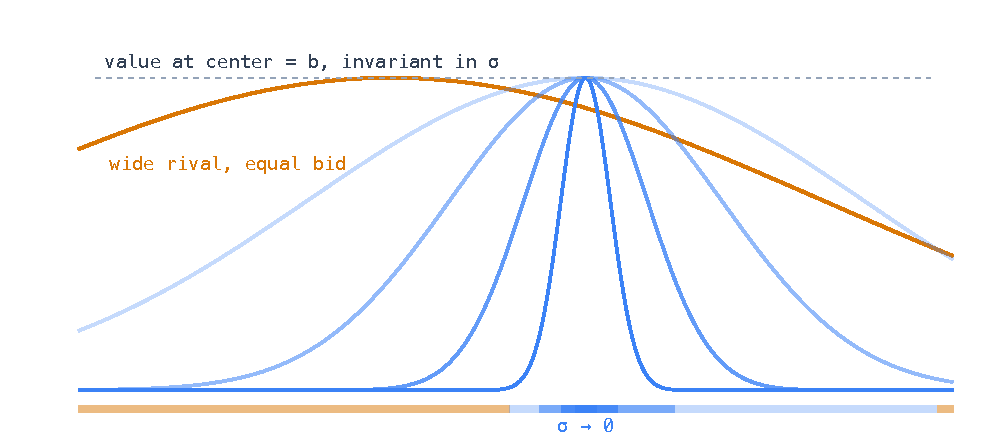
\includegraphics[keepaspectratio,alt={Shrinking \textbackslash sigma at a fixed center against a wide rival with equal bid. The value at the center is b for every \textbackslash sigma, while territory off-center collapses; in the limit the advertiser competes at one point only, on bid alone.}]{vcg-fig3.pdf}}
\caption{Shrinking \(\sigma\) at a fixed center against a wide rival
with equal bid. The value at the center is b for every \(\sigma\), while
territory off-center collapses; in the limit the advertiser competes at
one point only, on bid alone.}
\end{figure}

\subsection{Exact Vickrey}\label{exact-vickrey}

At a query point that is every advertiser's shared center, the Gaussian
factor is \texttt{exp(0)\ =\ 1} for every bidder, so reported value is
the bid. The winner is a highest bidder
(\texttt{winner\_maximizes\_bid\_of\_common\_center}), the Clarke pivot
equals the highest competing bid
(\texttt{vcgPayment\_common\_center\_second\_price}), and every loser
pays nothing (\texttt{vcgPayment\_eq\_zero\_of\_loser}). That is
Vickrey's sealed-bid second-price auction, allocation and payment both.
A keyword auction is what the embedding auction does at a point.

\section{Optimality}\label{optimality}

Pointwise welfare maximization integrates. For any measure over queries,
expected welfare under the score-argmax allocation weakly dominates
expected welfare under any rule the expectation operator evaluates,
power-diagram or not (\texttt{integral\_efficiency},
\texttt{gaussian\_optimality}; the theorem statements carry the exact
quantifiers). \texttt{gaussian\_vcg\_weakly\_dominates} conjoins the
three properties: welfare-optimal, dominant-strategy incentive
compatible, equilibrium-efficient. The last is the welfare guarantee
evaluated at truthful play, which \texttt{vcg\_strategyproof} certifies
as a Nash equilibrium. Inside the game, a truthful report weakly
dominates every deviation (\texttt{vcg\_dsic}); across allocation rules,
the mechanism's expected welfare weakly dominates every rival the
operator evaluates. The same order certifies the advertiser's best
strategy and the platform's best mechanism.

The artifact separately proves the equilibrium-decomposition theorem of
\href{https://arxiv.org/abs/1603.04641}{Ghani, Hedges, Winschel and Zahn
(2018)}. In their open games, where large games compose from smaller
ones, an equilibrium of the composite induces equilibria of the
components (\texttt{composed\_equilibria\_decompose}). Whether DSIC
composes the same way remains open, and the formalization records it as
open instead of assuming it.

Welfare, as the \hyperref[model]{Model} defines it, means willingness to
pay. A true value \(b \cdot  \exp(-\|x-c^{*}\|^{2}/\sigma ^{*2})\) is
what a conversion at query \texttt{x} is worth to the advertiser, so
pointwise welfare maximization routes every query to the bidder willing
to pay the most there, and the incentive theorems keep the declared
curves honest about where that willingness lives. The guarantee is also
dimension-free, and the keyword language is not. A keyword is a point
report whose territory vanishes in high dimension, so covering an
embedding space with keywords takes exponentially many reports, while a
Gaussian covers a region with three numbers.

\begin{figure}
\centering
\pandocbounded{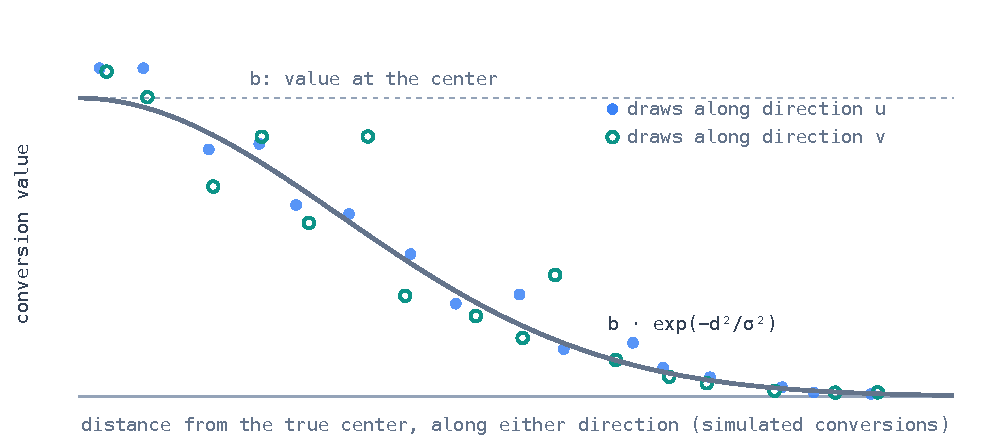
\includegraphics[keepaspectratio,alt={Simulated conversion values against distance from the true center, drawn along two directions of embedding space. Preferences need not be Gaussian for the model to be right about what a report can say: a peak and a width are all an advertiser can declare, and the isotropic Gaussian, equal weight in every dimension, is the maximum-entropy curve those two numbers justify.}]{vcg-fig5.pdf}}
\caption{Simulated conversion values against distance from the true
center, drawn along two directions of embedding space. Preferences need
not be Gaussian for the model to be right about what a report can say: a
peak and a width are all an advertiser can declare, and the isotropic
Gaussian, equal weight in every dimension, is the maximum-entropy curve
those two numbers justify.}
\end{figure}

The weak-order chain uses one modeling assumption,
\texttt{QueryMeasure.integral\_mono}: a monotone expectation operator
respects pointwise inequality (no normalization or probability mass
required). Strict expected comparisons additionally carry
\texttt{PositiveAt} or \texttt{PositiveOn}, stating that the operator
detects a contested point or region. These are structural hypotheses,
not Lean \texttt{axiom}s. \texttt{QueryMeasure.dirac} and
\texttt{QueryMeasure.ofWeightedFinset} construct the operator. A finite
weighted query log constructs the strictness witness whenever a
contested region contains a logged query of positive weight. A
measure-theoretic integral satisfies the corresponding interfaces on
functions and positive-mass regions it can evaluate. Keeping the
operator abstract lets the theorems quantify over query distributions
instead of fixing one, and each theorem carries the exact strength it
uses.

\section{Related Work}\label{related-work}

\subsection{LLM Ad Auctions}\label{llm-ad-auctions}

\href{https://arxiv.org/abs/2311.07601}{Feizi, Hajiaghayi, Rezaei and
Shin (2025)} survey the design space as four modules (modification,
bidding, prediction, auction) and leave open how the pieces sustain an
ad ecosystem. The idea of an auction inside the generation begins with
\href{https://arxiv.org/abs/2310.10826}{Dütting, Mirrokni, Paes Leme, Xu
and Zuo (2024)}, who aggregate advertisers' token distributions into the
reply and price the result through a monotonicity condition.
\href{https://arxiv.org/abs/2404.08126}{Dubey, Feng, Kidambi, Mehta and
Wang (2024)} auction placements inside an LLM-written summary of the
ads. MOSAIC and the retrieval-time mechanism are later points on that
line; all of them keep the ad inside the text the model emits.

\href{https://arxiv.org/abs/2405.05905}{Soumalias, Curry and Seuken
(2025)} give the prior LLM ad mechanism with dominant-strategy
guarantees. Their MOSAIC auction allocates the reply itself: advertiser
reward functions score candidate responses sampled from the model, and
softmax selects one. Computing the exact welfare-maximizing reply is out
of reach, so exact VCG is unavailable. The softmax allocation is instead
cyclically monotone, and
\href{https://doi.org/10.1016/0304-4068(87)90007-3}{Rochet (1987)} turns
cyclic monotonicity into dominant-strategy payments through a convex
potential. Auctioning an embedded intent point instead of the reply
shrinks the outcome space from token sequences to a finite set of known
advertisers. Exact VCG becomes one argmax plus one counterfactual
argmax, and the guarantees become simple enough for Lean to check.
Allocating a separate ad object also removes MOSAIC's deployment costs:
no multi-candidate generation per query, deterministic winners an
advertiser can budget against, and a discrete placement that can be
attributed and priced.

\href{https://arxiv.org/abs/2406.09459}{Hajiaghayi, Lahaie, Rezaei and
Shin (2024)} place the auction at retrieval time instead: their
mechanism retrieves ads probabilistically per discourse segment, by bid
and relevance, with incentive-compatible pricing. The outcome space is
far smaller than MOSAIC's, but the placement still lives inside the
generated text, and the winner is a draw rather than an argmax. The
geometric mechanism keeps the retrieval-time simplicity while making the
allocation deterministic and the ad a separate object.

\href{https://papers.ssrn.com/sol3/papers.cfm?abstract_id=6212838}{Alaei,
Makhdoumi and Malekian (2026)} share the geometric premise: a user is an
unknown preference vector, each advertiser a feature vector, match value
their inner product. Their platform learns the vector as the
conversation proceeds, trading a sharper estimate against the risk the
user leaves. The static \hyperref[model]{Model} holds that learning
dynamic fixed, and fixing the query point and the Gaussian family buys
the closed-form diagram and the compiled proof.

The other family bakes advertising into the model by training. Alibaba's
\href{https://arxiv.org/abs/2512.10551}{LLM-Auction} post-trains the
model with preference alignment to balance ad revenue against user
experience, encoding commercial incentives directly in the weights.
Training is the wrong cadence for an ad market: campaigns change hourly,
fine-tuning takes weeks, and retraining per campaign rotation costs more
than the campaign.

It is also the wrong trust surface. Outsiders cannot audit bias learned
in weights, and users cannot police it from inside either:
\href{https://arxiv.org/abs/2409.15436}{evaluators shown chatbot
responses with embedded ads} failed to detect the ads and preferred the
responses that contained them. The power-diagram mechanism is the
opposite limiting case. The scoring rule is public, the allocation is
its argmax, the incentive guarantee is a compiled theorem, and the audit
reduces to a build command.

\subsection{Semantic Matching}\label{semantic-matching}

Advertisers competing in a vector space is not new.
\href{https://arxiv.org/abs/1607.01869}{Grbovic et al.~(2016)} learned
joint query and ad embeddings to match ads beyond literal keywords, and
embedding-based retrieval is now standard ad-system infrastructure. In
that line the geometry supplies candidates or relevance features to a
separate auction. In the power diagram the distance function is the
valuation, and the auction is the geometry.

\subsection{Formalized Auctions}\label{formalized-auctions}

\href{https://arxiv.org/abs/1308.1779}{Caminati, Kerber, Lange and Rowat
(2013)} proved soundness of combinatorial Vickrey auctions in Isabelle
and generated verified executable code.
\href{https://arxiv.org/abs/1502.04052}{Barthe, Gaboardi, Gallego Arias,
Hsu, Roth and Strub (2015)} verified incentive compatibility for VCG in
a probabilistic relational calculus, and
\href{https://github.com/jouvelot/mech.v}{Jouvelot and Gallego Arias
(2022)} built mech.v, a Coq library that proves VCG's incentive
properties generically and refines an online-advertising VCG down to
that specification. Formalized VCG is not new, and neither is a verified
online-ad mechanism. What \hyperref[formalization]{this artifact} adds
is the object: the verified allocation is a partition of a vector space,
and the same artifact that checks truthfulness checks its identification
as a power diagram. Kerber, Lange and Rowat
(\href{https://doi.org/10.1016/j.jmateco.2016.06.005}{2016}) formalized
Vickrey's auction in Isabelle and argued mechanized reasoning should be
ordinary practice in economic theory;
\href{https://arxiv.org/abs/1603.04641}{Ghani, Hedges, Winschel and Zahn
(2018)} rebuilt game theory compositionally so that mechanisms assemble
from smaller games. The artifact extends the practice from a discrete
allocation rule to a geometric one.

\subsection{Filters and Reserves}\label{filters-and-reserves}

\href{https://arxiv.org/abs/2310.03702}{Hartline, Hoy and Taggart
(2023)} show competitive efficiency survives reserve pricing. The same
holds trivially for any pre-auction relevance filter, since welfare
maximization restricted to a nonempty eligible set is welfare
maximization on that set
(\texttt{tau\_preserves\_efficiency\_among\_eligible}). Revenue also
lives in reserves. The Clarke pivot collects only the runner-up's
implied value, zero when a winner is unopposed, and a reserve puts a
price floor under exactly those impressions.

\section{Limits}\label{limits}

{\def\LTcaptype{none} % do not increment counter
\begin{longtable}[]{@{}
  >{\raggedright\arraybackslash}p{(\linewidth - 2\tabcolsep) * \real{0.5000}}
  >{\raggedright\arraybackslash}p{(\linewidth - 2\tabcolsep) * \real{0.5000}}@{}}
\toprule\noalign{}
\begin{minipage}[b]{\linewidth}\raggedright
Element
\end{minipage} & \begin{minipage}[b]{\linewidth}\raggedright
In the formalization
\end{minipage} \\
\midrule\noalign{}
\endhead
\bottomrule\noalign{}
\endlastfoot
Embedding space \texttt{E} & any real inner product space; dimension
unconstrained \\
Advertisers & arbitrary finite type; no bound on the count \\
Query distribution & universally quantified expectation operator; one
assumption, monotonicity \\
Utility & quasilinear; no budget constraints \\
True valuations & isotropic Gaussian family \\
Deviations & any \((\mathrm{center}, \sigma , \mathrm{bid})\) triple \\
Rival allocation rules & any rule the expectation operator evaluates \\
Winners per query & exactly one; ties broken by fixed enumeration \\
\end{longtable}
}

\emph{Single winner.} Slates, pacing, and cross-impression externalities
are outside the model.

\emph{No budgets.} Budget-constrained clearing has known structure (with
fixed impression quotas it is
\href{https://arxiv.org/abs/2106.14730}{semi-discrete optimal
transport}, whose solution is again a power diagram; monetary budgets
are harder, since spend depends on runner-up values, not cell mass), but
its incentives and dynamics are open. \hyperref[simulations]{The
simulations} suggest the dynamics are where the difficulty lives.

\emph{Gaussian truth.} The Gaussian family is a bidding language, and
every deployed auction clears one. The reigning language is the keyword,
the \(\sigma\) \(\rightarrow\) 0 point mass of this same family. A
bidding language buys expressiveness against clearing cost, the central
tradeoff of the combinatorial-auction literature
(\href{https://doi.org/10.1145/352871.352872}{Nisan, 2000}). On that
frontier the isotropic Gaussian is the most expressive language
currently known to admit sublinear clearing, exact VCG, and a compiled
proof. Anisotropic preferences (elliptical rather than spherical reach)
stay computable at O(N) per query but break the bridge lemma as stated;
whether a lifted variant survives for quadratic-form preferences is the
natural next theorem, since Aurenhammer's lift already accommodates
general quadrics. Mixtures turn the score into a log-sum-exp whose
bisectors admit no fixed-dimension lift, and the clearing speed and the
proof leave with the geometry.

\emph{Frozen embedder.} We hold the embedding model fixed. Retraining or
replacing it moves every conversation point and every declared center at
once, invalidating reports with no advertiser misreporting anything;
re-declaration cadence is an operational question the model does not
pose.

\emph{Statics only.} Nothing in the artifact says bidding dynamics
converge. \hyperref[simulations]{The simulations} study the dynamics
empirically; a formal convergence or limit-cycle result would be a
separate paper's contribution.

\section{Discussion}\label{discussion}

Why now? Four implications answer, outside the theorems but shaped by
them. Each names its evidence.

\emph{The minimum viable firm shrinks.}
\href{https://doi.org/10.1111/j.1468-0335.1937.tb00002.x}{Coase (1937)}
set the boundary of the firm where the cost of transacting outside it
exceeds the cost of organizing inside, so the boundary moves when
transaction costs do. A recent literature asks whether AI agents
collapse those costs market-wide;
\href{https://www.nber.org/books-and-chapters/economics-transformative-ai/coasean-singularity-demand-supply-and-market-design-ai-agents}{Shahidi,
Rusak, Manning, Fradkin and Horton (2025)} call the limit the Coasean
singularity. But the collapse runs through discovery, because small
firms survive by specialization, and specialization only pays where
specialists can be found. The market on offer prices discovery for
scale, because keyword advertising amortizes vocabulary research,
bidding infrastructure, and autobidding retainers only over large
budgets, and training-based placement gates entry on the platform's
fine-tuning calendar. The market specialists need prices a campaign at
one report, allocates efficiently, admits any campaign size, and can
discover a more diverse population of firms.

\emph{So positioning becomes the bidding language.} The power-diagram
mechanism replaces the keyword portfolio with one report per campaign.
The report says who the customer is, how far the claim extends, and what
the fit is worth. This is the market position statement made formal, and
every marketer already writes one, because the position statement is the
first document a campaign produces. Advertisers think in positioning and
users think in problems, so keywords became the middle vocabulary both
sides had to learn, the compression lost the situation that makes a
customer the right fit, and the platform that authored the vocabulary
charged rent for the translation. But this report drops the translation,
and adopting it strands no keyword buyer, because in
\hyperref[keywords-recovered]{Keywords Recovered} the keyword auction
embeds as one point of the general mechanism. The declaration also
binds, because the incentive theorem covers all three fields, so no
misdeclaration profits and the allocation-changing ones cost. Richer
bidding languages have paid before;
\href{https://ojs.aaai.org/aimagazine/index.php/aimagazine/article/view/2054}{Sandholm
(2007)} cleared \$35 billion of sourcing through expressive
combinatorial bids and reported \$4.4 billion of hard-dollar savings.
But that evidence comes from procurement, so advertising is the untested
extension, and a deployment would measure whether the one-report
campaign lowers the minimum profitable campaign size and shifts entry
toward smaller firms.

\emph{The keyword tax shrinks with it.}
\href{https://web.stanford.edu/~jdlevin/Papers/OnlineAds.pdf}{Levin and
Milgrom (2010)} call the tax conflation, pooling heterogeneous items
into one auction. A keyword bin is conflation at the item-definition
layer, where the climbing specialist pays to compete on pelvic-floor
queries it will never convert. But heterogeneous reach un-conflates,
because a tight specialist wins where its reported value leads without
submitting a separate bid for every nearby keyword. The geometry section
proves the carving, and \hyperref[simulations]{the simulations} estimate
the surplus it recovers in a synthetic fifteen-advertiser market. But
those estimates have to clear Levin and Milgrom's own counterweight,
since finer segmentation can thin markets and weaken price discovery.
The ecological hypothesis pushes back, because a finite keyword
vocabulary routes demand only to businesses it has words for, while a
continuous positioning space can host any firm a center and a reach can
describe, so the richer language admits a more diverse population of
discoverable firms. And the pattern has retail precedent, because when
online catalogs lowered discovery costs,
\href{https://sloanreview.mit.edu/article/from-niches-to-riches-anatomy-of-the-long-tail/}{Brynjolfsson,
Hu and Smith (2006)} measured demand shifting into the niche tail.

\emph{But the collapse runs on elicited information.} Cheap coordination
does not supply the information coordination needs, because dispersed
knowledge must be elicited
(\href{https://www.econlib.org/library/Essays/hykKnw.html}{Hayek
(1945)}), and advertising is the market that produces the
who-serves-whom half of it;
\href{https://www.journals.uchicago.edu/doi/abs/10.1086/260231}{Nelson
(1974)} founded the economics of advertising on its information content.
The stakes run to the whole margin, because the \hyperref[model]{Model}
prices true value as margin times conversion rate, so the ceiling on
what an advertiser will pay for discovery is everything the sale clears,
and the mechanism sets which share changes hands. So the incentives of
the mechanism that clears it set the quality of that information.
Conflated auctions produce conflated knowledge, weights produce
knowledge nobody can audit, and in the power diagram, truthful reporting
is the compiled incentive. The agent economy therefore inherits the
incentives of whatever clears its discovery.

The open problems:

\begin{itemize}
\tightlist
\item
  whether DSIC composes across open games (recorded open in the
  artifact, with the equilibrium half proved)
\item
  whether the bridge lemma reformulates for anisotropic preferences
\item
  whether bidding dynamics converge once budgets enter the mechanism
\end{itemize}

The open measurements:

\begin{itemize}
\tightlist
\item
  what it costs an advertiser to estimate a report
\item
  whether the richer bidding language cuts campaign setup cost and
  misallocation
\item
  whether specialist surplus, market thickness, and small-firm entry
  hold up together
\item
  whether allocations stay stable after embedder recalibration
\end{itemize}

\section*{Artifacts}\label{artifacts}
\addcontentsline{toc}{section}{Artifacts}

\subsection*{Formalization}\label{formalization}
\addcontentsline{toc}{subsection}{Formalization}

The formalization is at
\href{https://github.com/kimjune01/auction-proof}{github.com/kimjune01/auction-proof},
archived as \href{https://doi.org/10.5281/zenodo.21214697}{DOI
10.5281/zenodo.21214697}, AGPL-3.0, \href{https://lean-lang.org/}{Lean
4} (v4.29.0-rc6) with
\href{https://github.com/leanprover-community/mathlib4}{Mathlib}.
Verification:

\begin{verbatim}
lake exe cache get
lake build
\end{verbatim}

Zero \texttt{sorry}, and no trusted axiom of our own.
\texttt{\#print\ axioms} on every theorem below returns only Lean's
three standard background axioms (\texttt{propext},
\texttt{Classical.choice}, \texttt{Quot.sound}), because the single
modeling assumption is a \texttt{QueryMeasure} typeclass that concrete
instances discharge by proof. The claims-to-theorems map:

{\def\LTcaptype{none} % do not increment counter
\begin{longtable}[]{@{}
  >{\raggedright\arraybackslash}p{(\linewidth - 4\tabcolsep) * \real{0.2800}}
  >{\raggedright\arraybackslash}p{(\linewidth - 4\tabcolsep) * \real{0.4700}}
  >{\raggedright\arraybackslash}p{(\linewidth - 4\tabcolsep) * \real{0.2500}}@{}}
\toprule\noalign{}
\begin{minipage}[b]{\linewidth}\raggedright
Claim
\end{minipage} & \begin{minipage}[b]{\linewidth}\raggedright
Lean theorem
\end{minipage} & \begin{minipage}[b]{\linewidth}\raggedright
File
\end{minipage} \\
\midrule\noalign{}
\endhead
\bottomrule\noalign{}
\endlastfoot
score = log(reported value) & \texttt{score\_eq\_log\_reportedVal} &
Efficiency.lean \\
winner maximizes true welfare & \texttt{winner\_maximizes\_welfare} &
Efficiency.lean \\
truthful reporting is dominant & \texttt{vcg\_dsic} &
Strategyproof.lean \\
no allocation rule beats VCG & \texttt{gaussian\_optimality} &
GaussianOptimality.lean \\
capstone conjunction & \texttt{gaussian\_vcg\_weakly\_dominates} &
GaussianOptimality.lean \\
equal-\(\sigma\) power diagram, hyperplane bisectors, winner minimizes
power distance & \texttt{score\_le\_iff\_powerDist\_le},
\texttt{score\_sub\_affine}, \texttt{winner\_minimizes\_powerDist} &
PowerDiagram.lean \\
variable-\(\sigma\) power diagram via paraboloid lift &
\texttt{liftedPowerDist\_paraboloid},
\texttt{winner\_minimizes\_liftedPowerDist} & PowerDiagram.lean \\
keyword limit & \texttt{keyword\_is\_degenerate\_limit} &
VectorSpace.lean \\
exact Vickrey at a keyword point &
\texttt{vcgPayment\_common\_center\_second\_price} & SecondPrice.lean \\
losers pay nothing & \texttt{vcgPayment\_eq\_zero\_of\_loser} &
Strategyproof.lean \\
\end{longtable}
}

\subsection*{Exchange}\label{exchange}
\addcontentsline{toc}{subsection}{Exchange}

\href{https://github.com/kimjune01/vectorspace-adserver}{vectorspace-adserver}
implements the mechanism as an open-source exchange,
\href{https://vectorspace.exchange/}{live at vectorspace.exchange} and
archived as \href{https://doi.org/10.5281/zenodo.21365911}{DOI
10.5281/zenodo.21365911}: the scoring rule, the argmax allocation, and
the Clarke pivot.

\subsection*{Simulations}\label{simulations}
\addcontentsline{toc}{subsection}{Simulations}

\href{https://github.com/kimjune01/openauction/tree/v3.4/cmd/simulate}{openauction/cmd/simulate},
archived as \href{https://doi.org/10.5281/zenodo.21366035}{DOI
10.5281/zenodo.21366035}, runs the market on real
\href{https://huggingface.co/BAAI/bge-small-en-v1.5}{BGE-small-en-v1.5}
embeddings: fifteen advertisers, 62 queries, 50 randomized trials,
keyword and embedding clearing compared head to head.
\href{https://june.kim/keyword-tax}{Keyword Tax} and
\href{https://june.kim/relocation-fees}{Relocation Fees} report the
results.

\subsection*{Explorer}\label{explorer}
\addcontentsline{toc}{subsection}{Explorer}

\href{https://june.kim/vectorspace-ads/}{vectorspace-ads} renders the
allocation live, archived as
\href{https://doi.org/10.5281/zenodo.21365798}{DOI
10.5281/zenodo.21365798}: drag a center or raise a bid and the
territories shift.

\section*{Acknowledgments}\label{acknowledgments}
\addcontentsline{toc}{section}{Acknowledgments}

Conversations with Sébastien Lahaie and Mohammad Hajiaghayi sharpened
the mechanism-design framing, and Sébastien pointed me to MOSAIC.
Errors, and the claims, are mine.

\section*{Disclosures}\label{disclosures}
\addcontentsline{toc}{section}{Disclosures}

\emph{LLM use.} This paper and its artifact were produced with large
language models via \href{https://claude.ai/claude-code}{Claude Code}.
The author directed the research and reviewed every claim; agents wrote
the Lean proofs, generated the figures, and drafted the prose. A
separate model ran an adversarial review of the prose against the
formalization. No guarantee in this paper rests on any model's judgment:
the artifact type-checks with zero \texttt{sorry}, and verification
reduces to \texttt{lake\ build}.

\emph{Funding.} Self-funded independent research. No external funding,
no employer direction, no advertiser or platform relationship.

\section*{References}\label{references}
\addcontentsline{toc}{section}{References}

Alaei, S., Makhdoumi, A., and Malekian, A. (2026). Dynamic Learning and
Optimal Advertising Mechanism for LLM Platforms.
\href{https://papers.ssrn.com/sol3/papers.cfm?abstract_id=6212838}{SSRN
working paper}.

Aurenhammer, F. (1987). Power Diagrams: Properties, Algorithms and
Applications. \href{https://doi.org/10.1137/0216006}{\emph{SIAM Journal
on Computing} 16(1), 78--96}.

Barthe, G., Gaboardi, M., Gallego Arias, E. J., Hsu, J., Roth, A., and
Strub, P.-Y. (2015). Computer-Aided Verification in Mechanism Design.
\href{https://arxiv.org/abs/1502.04052}{arXiv:1502.04052}.

Brynjolfsson, E., Hu, Y. J., and Smith, M. D. (2006). From Niches to
Riches: Anatomy of the Long Tail.
\href{https://sloanreview.mit.edu/article/from-niches-to-riches-anatomy-of-the-long-tail/}{\emph{Sloan
Management Review} 47(4), 67--71}.

Caminati, M. B., Kerber, M., Lange, C., and Rowat, C. (2013). Proving
Soundness of Combinatorial Vickrey Auctions and Generating Verified
Executable Code.
\href{https://arxiv.org/abs/1308.1779}{arXiv:1308.1779}.

Caplan, P. C. (2021). Higher-Dimensional Power Diagrams for
Semi-Discrete Optimal Transport.
\href{https://arxiv.org/abs/2106.14730}{arXiv:2106.14730}.

Clarke, E. H. (1971). Multipart Pricing of Public Goods.
\href{https://doi.org/10.1007/BF01726210}{\emph{Public Choice} 11,
17--33}.

Coase, R. H. (1937). The Nature of the Firm.
\href{https://doi.org/10.1111/j.1468-0335.1937.tb00002.x}{\emph{Economica}
4(16), 386--405}.

Dubey, K. A., Feng, Z., Kidambi, R., Mehta, A., and Wang, D. (2024).
Auctions with LLM Summaries.
\href{https://arxiv.org/abs/2404.08126}{arXiv:2404.08126}.

Dütting, P., Mirrokni, V., Paes Leme, R., Xu, H., and Zuo, S. (2024).
Mechanism Design for Large Language Models.
\href{https://arxiv.org/abs/2310.10826}{arXiv:2310.10826}.

Edelman, B., Ostrovsky, M., and Schwarz, M. (2007). Internet Advertising
and the Generalized Second-Price Auction: Selling Billions of Dollars
Worth of Keywords.
\href{https://www.aeaweb.org/articles?id=10.1257/aer.97.1.242}{\emph{American
Economic Review} 97(1), 242--259}.

Feizi, S., Hajiaghayi, M., Rezaei, K., and Shin, S. (2025). Online
Advertisements with LLMs: Opportunities and Challenges.
\href{https://arxiv.org/abs/2311.07601}{arXiv:2311.07601}.

Ghani, N., Hedges, J., Winschel, V., and Zahn, P. (2018). Compositional
Game Theory. \href{https://arxiv.org/abs/1603.04641}{LICS '18;
arXiv:1603.04641}.

Grbovic, M., Djuric, N., Radosavljevic, V., Silvestri, F., Baeza-Yates,
R., Feng, A., Ordentlich, E., Yang, L., and Owens, G. (2016). Scalable
Semantic Matching of Queries to Ads in Sponsored Search Advertising.
\href{https://arxiv.org/abs/1607.01869}{SIGIR '16; arXiv:1607.01869}.

Groves, T. (1973). Incentives in Teams.
\href{https://doi.org/10.2307/1914085}{\emph{Econometrica} 41(4),
617--631}.

Hajiaghayi, M., Lahaie, S., Rezaei, K., and Shin, S. (2024). Ad Auctions
for LLMs via Retrieval Augmented Generation.
\href{https://arxiv.org/abs/2406.09459}{arXiv:2406.09459}.

Hartline, J., Hoy, D., and Taggart, S. (2023). Robust Analysis of
Auction Equilibria.
\href{https://arxiv.org/abs/2310.03702}{arXiv:2310.03702}.

Hayek, F. A. (1945). The Use of Knowledge in Society.
\href{https://www.econlib.org/library/Essays/hykKnw.html}{\emph{American
Economic Review} 35(4), 519--530}.

Hotelling, H. (1929). Stability in Competition.
\href{https://doi.org/10.2307/2224214}{\emph{The Economic Journal}
39(153), 41--57}.

Jouvelot, P., and Gallego Arias, E. J. (2022). mech.v: A Coq
Formalization of Mechanism Design.
\href{https://github.com/jouvelot/mech.v}{GitHub repository}.

Kerber, M., Lange, C., and Rowat, C. (2016). An Introduction to
Mechanized Reasoning.
\href{https://doi.org/10.1016/j.jmateco.2016.06.005}{\emph{Journal of
Mathematical Economics} 66, 26--39}.

Lahaie, S., and Pennock, D. M. (2007). Revenue Analysis of a Family of
Ranking Rules for Keyword Auctions.
\href{https://doi.org/10.1145/1250910.1250918}{EC '07, 50--56}.

Levin, J., and Milgrom, P. (2010). Online Advertising: Heterogeneity and
Conflation in Market Design.
\href{https://web.stanford.edu/~jdlevin/Papers/OnlineAds.pdf}{\emph{American
Economic Review} 100(2), 603--607}.

Nelson, P. (1974). Advertising as Information.
\href{https://www.journals.uchicago.edu/doi/abs/10.1086/260231}{\emph{Journal
of Political Economy} 82(4), 729--754}.

Nisan, N. (2000). Bidding and Allocation in Combinatorial Auctions.
\href{https://doi.org/10.1145/352871.352872}{EC '00}.

Nisan, N., Roughgarden, T., Tardos, É., and Vazirani, V. V.,
eds.~(2007). Algorithmic Game Theory.
\href{https://doi.org/10.1017/CBO9780511800481}{Cambridge University
Press}.

Rochet, J.-C. (1987). A Necessary and Sufficient Condition for
Rationalizability in a Quasi-Linear Context.
\href{https://doi.org/10.1016/0304-4068(87)90007-3}{\emph{Journal of
Mathematical Economics} 16(2), 191--200}.

Sandholm, T. (2007). Expressive Commerce and Its Application to
Sourcing: How We Conducted \$35 Billion of Generalized Combinatorial
Auctions.
\href{https://ojs.aaai.org/aimagazine/index.php/aimagazine/article/view/2054}{\emph{AI
Magazine} 28(3)}.

Shahidi, P., Rusak, G., Manning, B. S., Fradkin, A., and Horton, J. J.
(2025). The Coasean Singularity? Demand, Supply, and Market Design with
AI Agents. In \emph{The Economics of Transformative AI}.
\href{https://www.nber.org/books-and-chapters/economics-transformative-ai/coasean-singularity-demand-supply-and-market-design-ai-agents}{NBER}.

Soumalias, E., Curry, M. J., and Seuken, S. (2025). Truthful Aggregation
of LLMs with an Application to Online Advertising.
\href{https://arxiv.org/abs/2405.05905}{arXiv:2405.05905}.

Tang, B. J., Sun, K., Curran, N. T., Schaub, F., and Shin, K. G. (2024).
Ads that Talk Back: Implications and Perceptions of Injecting
Personalized Advertising into LLM Chatbots.
\href{https://arxiv.org/abs/2409.15436}{arXiv:2409.15436}.

Vickrey, W. (1961). Counterspeculation, Auctions, and Competitive Sealed
Tenders. \href{https://doi.org/10.2307/2977633}{\emph{Journal of
Finance} 16(1), 8--37}.

Zhao, C., Hu, Q., Song, S., Chen, D., Zhu, H., Xu, J., and Zheng, B.
(2025). LLM-Auction: Generative Auction towards LLM-Native Advertising.
\href{https://arxiv.org/abs/2512.10551}{arXiv:2512.10551}.
